\documentclass{article}
\usepackage{amsmath,amsfonts,amsthm,amssymb}
\usepackage{fullpage,fancyhdr}
\usepackage[pdftex]{graphicx}
\usepackage[usenames,dvipsnames]{color}
\usepackage{listings}
\usepackage{courier}
\usepackage{ifthen}
\usepackage{setspace}
\usepackage{lastpage}
\usepackage{extramarks}
\usepackage{chngpage}
\usepackage{soul}
\usepackage{graphicx,float,wrapfig}
\usepackage{epstopdf}
\usepackage{geometry}
\usepackage{pdfcolmk}
\usepackage{hyperref}
\DeclareGraphicsRule{.tif}{png}{.png}{`convert #1 `dirname #1`/`basename #1 .tif`.png}

\definecolor{lightgray}{gray}{0.5}
\definecolor{darkgray}{gray}{0.3}
\definecolor{MyDarkGreen}{rgb}{0.0,0.4,0.0}

\topmargin=-0.45in      %
\evensidemargin=0in     %
\oddsidemargin=0in      %
\textwidth=6.5in        %
\textheight=9.0in       %
\headsep=0.25in         %

\pagestyle{fancyplain}
 
\fancyhf{}
 
\lhead{\fancyplain{}{Michael Carroll}}
\chead{\fancyplain{}{ELEC6230 - Parallel Processing}}
\rhead{\fancyplain{}{\today}}
\rfoot{\fancyplain{}{\thepage\ of \pageref{LastPage}}}

\sloppy
\setlength{\parindent}{0pt}

\lstloadlanguages{C++}
\lstset{
language=C++,
frame=single,
basicstyle=\ttfamily,
keywordstyle=[1]\color{Blue}\bf,
keywordstyle=[2]\color{Purple},
keywordstyle=[3]\color{Blue}\underbar,
identifierstyle=,
numbers=left,
numberstyle=\tiny\color{Blue},
stepnumber=5,
morekeywords={printf,atoi,omp,parallel,shared,schedule,reduction},
morekeywords=[2]{gettimeofday,matrixSize,omp_get_wtime,omp_set_num_threads}
}

% Alter some LaTeX defaults for better treatment of figures:
% See p.105 of "TeX Unbound" for suggested values.
% See pp. 199-200 of Lamport's "LaTeX" book for details.
%   General parameters, for ALL pages:
\renewcommand{\topfraction}{0.9}	% max fraction of floats at top
\renewcommand{\bottomfraction}{0.8}	% max fraction of floats at bottom
%   Parameters for TEXT pages (not float pages):
\setcounter{topnumber}{2}
\setcounter{bottomnumber}{2}
\setcounter{totalnumber}{4}     % 2 may work better
\setcounter{dbltopnumber}{2}    % for 2-column pages
\renewcommand{\dbltopfraction}{0.9}	% fit big float above 2-col. text
\renewcommand{\textfraction}{0.07}	% allow minimal text w. figs
%   Parameters for FLOAT pages (not text pages):
\renewcommand{\floatpagefraction}{0.7}	% require fuller float pages
% N.B.: floatpagefraction MUST be less than topfraction !!
\renewcommand{\dblfloatpagefraction}{0.7}	% require fuller float pages

% remember to use [htp] or [htpb] for placement

\title{ELEC6230 Homework 9\\
{\large \begin{par}
Answers to Parallel Processing Homework 9
\end{par} \vspace{1em}
}}
\author{Michael J. Carroll}

\begin{document}
\maketitle

\section*{Part 1 Results}
\begin{par}
For Homework 9, I reimplemented the previous week's homework assignment.  The addition for this week's code was the ability to cache matrix values from global memory into the much faster shared memory.  To accomplish this, each spot in two submatricies was copied from the global matricies by each thread in a block.  The multiplication was then performed over the block.  The results of using block size B = 4, 8, and 16 are included below, and compared to the previous results without using shared memory.  The code for this implementation is attached in Appendix A.\\
\\
The speedup from using the shared memory is significant.  The reason is that the processors can spend less time fetching from the memory (due to reduced latency), and more time performing the actual matrix multiplication.  The ratio of memory access to actual arithmetic is what defines the performance on the GPU processing.\\
\\
I additionally got to use the NVidia visual profiler to see where (if any) choke points existed in my code implementation.  While I didn't find any, I experimented with using the "\#pragma unroll" command on the inner for loop in the kernel.  The pragma did not provide any noticeable performance increase (under 0.5\%) in the GPU.\\
\\
Another interesting result is that the larger the block size, the higher the speedup.  This is counter to previous programming environments (OpenMP, MPI).  The GPU is more fully utilized (almost 100\% with a 16x16 block size) when more processes are added.  This is a good example of optimizing the block and grid sizes to the GPU's requirements.
\end{par}

\begin{table}
\begin{center}
\begin{tabular}[tbph]{| l | r | r | r | r |}
\hline
Program Type & Sequential & Parallel (4) & Parallel (8) & Parallel (16)  \\
\hline
Global Memory Implementation & 34.47 s & 19.96 s & 8.09 s & 5.75 \\
Shared Memory Implementation & 34.47 s & 5.41 s & 1.42 s & 0.85 s \\
\hline
\textbf{Speedup} & 1.00 & 6.37 & 24.27 & 40.55 \\ 
\hline
\end{tabular}
\caption{Parallel Speedup}
\end{center}
\end{table}

\section*{Part 2 Results}
\begin{par}
I was wholly unsuccessful in implementing Part 2 of the homework. \\
\\
Theoretically, the performance should increase as the window size increases, up to a point.  The Nvidia visual profiling tool revealed to me that not all of the shared memory was being used during the execution of the matrix multiplication.  Because of this, we can cache more into the the shared memory over the course of the operation of a single thread.\\
\\
By using as much shared memory as possible (and as a result using the fastest memory possible), we can further reduce the ratio of memory fetch time to actual execution instructions.  This would give additional performance enhancements, although not on the order of switching from global to shared memory.\\
\\
At a certain point, this performance would degrade as the shared memory would get full.  I would estimate that a window of 4x4 or 8x8 would give the best performance in terms of speedup while maintaining correctness.
\end{par}



\begin{figure}[htp]
	\begin{center}
	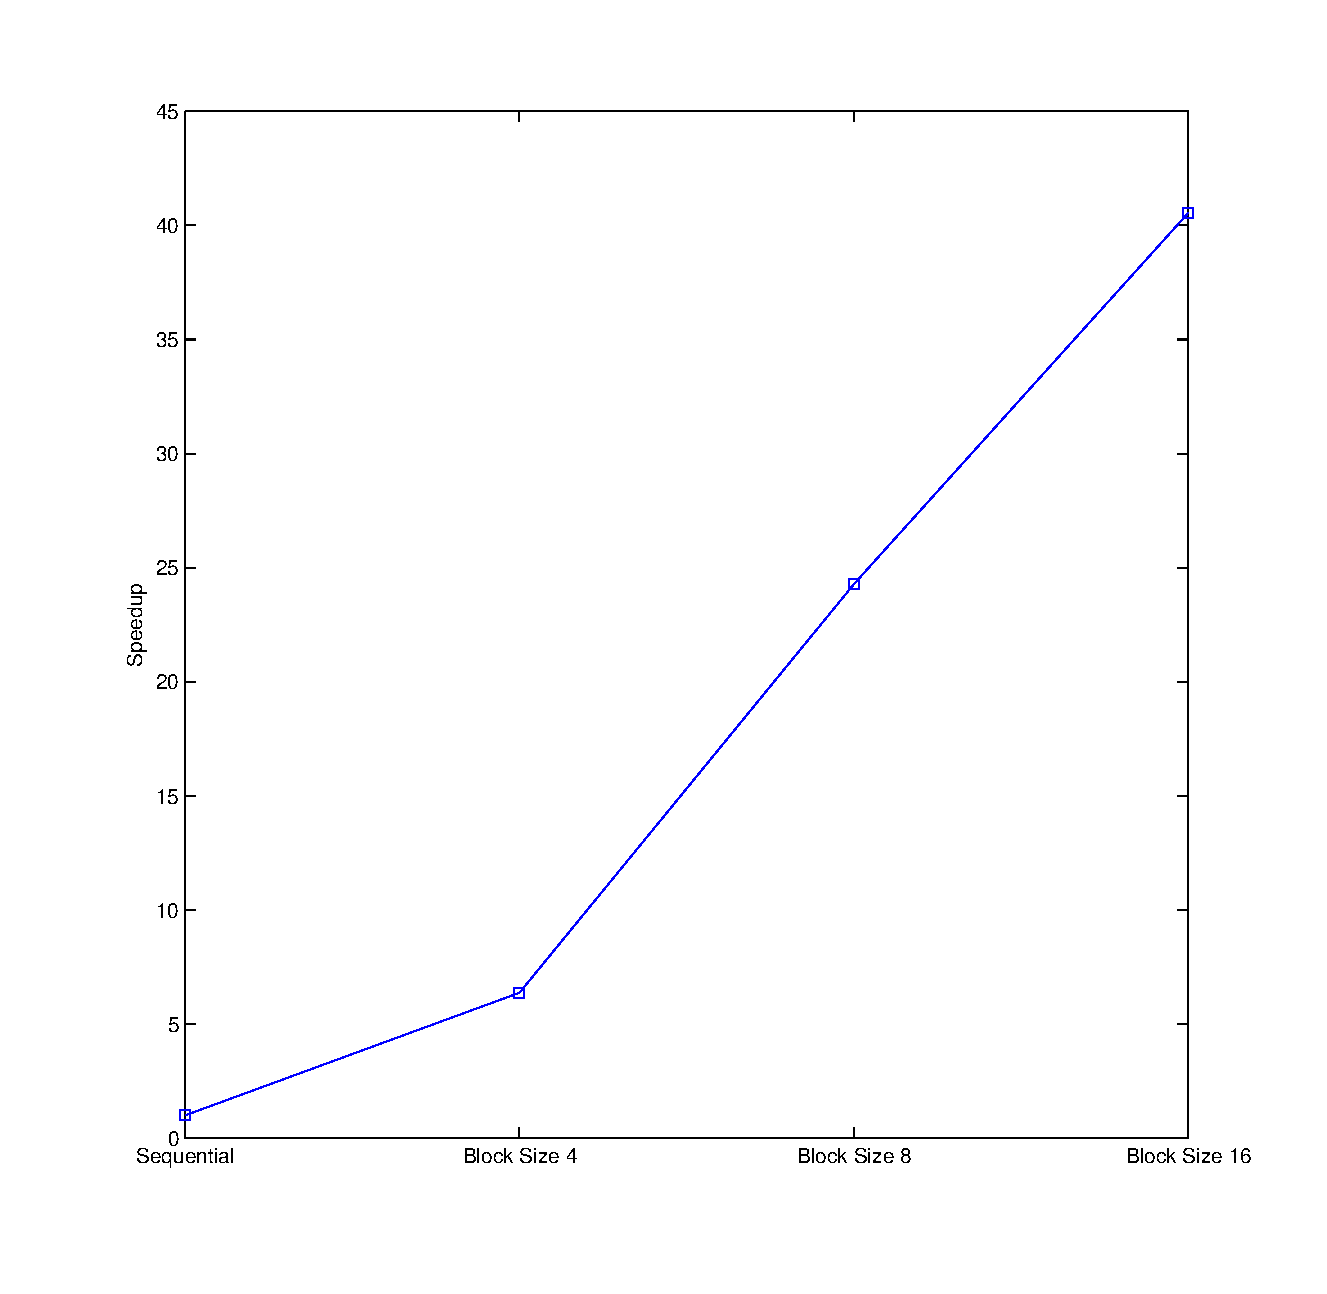
\includegraphics[width=5in]{speedup.eps}
	\caption{Speedup Plot}
	\label{fig:figure1}
	\end{center}
\end{figure}

\newpage
\section*{Appendix A - Global Memory CUDA Implementation}
\lstinputlisting{../multiply-block.cu}


\end{document}